%%%%%%%%%%%%%%%%%%%%%%%%%%%%%%%%%%%%%%%%%%%%%%%%%%%%%%%%%%%%%%%%%%%%%%%%%%%
%% This file is part of the book
%%
%% Algorithmic Graph Theory
%% http://code.google.com/p/graph-theory-algorithms-book/
%%
%% Copyright (C) 2009, 2010 Minh Van Nguyen <nguyenminh2@gmail.com>
%%
%% See the file COPYING for copying conditions.
%%%%%%%%%%%%%%%%%%%%%%%%%%%%%%%%%%%%%%%%%%%%%%%%%%%%%%%%%%%%%%%%%%%%%%%%%%%

%% graph G_1
\subfigure[$G_1$]{
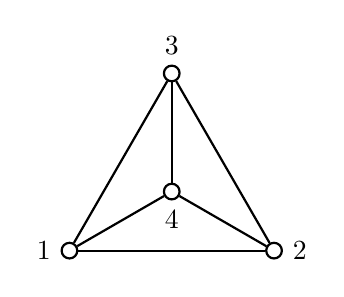
\begin{tikzpicture}
[nodedecorate/.style={shape=circle,inner sep=2pt,draw,thick},%
  linedecorate/.style={-,thick},%
  scale=1.5]
%% nodes or vertices
\foreach \nodename/\x/\y/\direction/\navigate in {
  1/-0.8660/-0.5/left/west, 2/0.8660/-0.5/right/east,
  3/0/1/above/north, 4/0/0/below/south}
{
  \node (\nodename) at (\x,\y) [nodedecorate] {};
  \node [\direction] at (\nodename.\navigate) [] {$\nodename$};
}
%% edges or lines
\path
\foreach \startnode/\endnode in {1/2, 1/3, 1/4, 2/3, 2/4, 3/4} {
  (\startnode) edge[linedecorate] node {} (\endnode)
};
\end{tikzpicture}
}
\quad
%%
%% graph G_2
\subfigure[$G_2$]{
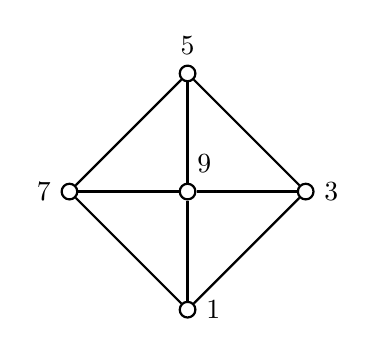
\begin{tikzpicture}
[nodedecorate/.style={shape=circle,inner sep=2pt,draw,thick},%
  linedecorate/.style={-,thick},%
  scale=1.5]
%% nodes or vertices
\foreach \nodename/\x/\y/\direction/\navigate in {
  1/0/-1/right/east, 3/1/0/right/east, 5/0/1/above/north,
  7/-1/0/left/west, 9/0/0/above right/north}
{
  \node (\nodename) at (\x,\y) [nodedecorate] {};
  \node [\direction] at (\nodename.\navigate) [] {$\nodename$};
}
%% edges or lines
\path
\foreach \startnode/\endnode in {1/3, 1/7, 1/9, 3/5, 3/9, 5/7, 5/9, 7/9} {
  (\startnode) edge[linedecorate] node {} (\endnode)
};
\end{tikzpicture}
}
\quad
%%
%% graph G_1 symmetric difference G_2
\subfigure[$G_1 \Delta G_2$]{
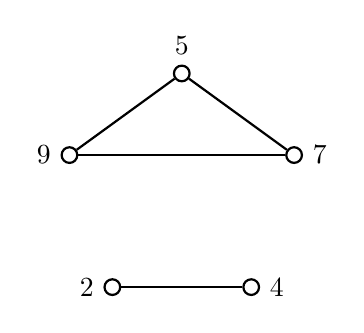
\begin{tikzpicture}
[nodedecorate/.style={shape=circle,inner sep=2pt,draw,thick},%
  linedecorate/.style={-,thick},%
  scale=1.5]
%% nodes or vertices
\foreach \nodename/\x/\y/\direction/\navigate in {
  2/-0.5877/-0.8090/left/west, 4/0.5877/-0.8090/right/east,
  5/0/1/above/north, 7/0.9510/0.3090/right/east,
  9/-0.9510/0.3090/left/west}
{
  \node (\nodename) at (\x,\y) [nodedecorate] {};
  \node [\direction] at (\nodename.\navigate) {$\nodename$};
}
%% edges or lines
\path
\foreach \startnode/\endnode in {2/4, 5/7, 5/9, 7/9} {
  (\startnode) edge[linedecorate] node {} (\endnode)
};
\end{tikzpicture}
}
